\documentclass[11pt]{article}
\usepackage[margin=1.05in]{geometry}
\usepackage{amsmath,amssymb}
\usepackage{graphicx}
\usepackage[colorlinks=true,linkcolor=blue!50!black,citecolor=blue!50!black,urlcolor=blue!50!black]{hyperref}
\usepackage{xcolor}
\graphicspath{{figs/}}
\setlength{\parskip}{2pt}
\emergencystretch=2em

\title{\bfseries Short-Horizon Kinetics of Causal-Entropic Forcing:\\ A Pre-Registered Signature, Audited and Dissolved\\ by Matched-Estimator Control}
\author{Anthony J.~Vasquez Sr.\\ \small The Temple of Two, Hilltown, Pennsylvania \\ \small \texttt{thetempleoftwo.com}}
\date{July 9, 2026 \quad (the v4 arc complete: v4.0--v4.3)}

\begin{document}
\maketitle

\begin{abstract}
Causal-entropic forcing (Wissner-Gross and Freer, 2013) drives a system toward states of maximal future path entropy. A prior study in this program found that in the conservative overdamped regime the force reduces to a $\tau$-tunable equilibrium: statics in disguise. Three pre-registered campaigns then tested whether the \emph{implementation} of such a force carries a kinetic signature invisible to statics, and the answer arrives only when they are read as one arc. Campaign v4.1 found an apparent short-horizon first-passage separation between an online (per-step sampled) force and its frozen conservative control (block-permutation $p \le 5\times10^{-4}$ at $\tau{=}0.25$ and $0.5$; Hedges' $g \approx 1.8$; the online arm slower), but its occupancy gate was malformed: as registered it compared a $\chi^2$-style \emph{distance} to a significance level as if the distance were a p-value, a gate incapable of failing. An independent audit caught this before publication, and every checkable quantity in the audit reproduced exactly against the raw data. Campaign v4.2, re-registered with gates demonstrably able to fail and with \emph{matched-estimator} arms (frozen and online at equal rollout count $M$, cache controlled, plus an $M$-sweep), dissolves the effect: at matched $M$ the arms are indistinguishable in first-passage kinetics ($p = 0.47$, $g = -0.32$), while the $M$-sweep shows the apparent v4.1 separation scaling with sampling roughness (slope $+0.63$ against $\log(1/M)$, $p = 5\times10^{-4}$). The mechanism is finite-sample estimator roughness, not the implementation. No coherent current appears in either arm, and a structural argument shows any force computed as the gradient of a scalar path-entropy field is conservative by construction. The kinetic axis therefore joins the static one: in this regime causal-entropic forcing is statics in disguise. A fourth campaign then repaired the one control that had been too weak to matter and used it to test the minimal non-conservative extension of the force, per-coordinate planning horizons whose curl is nonzero by construction; with the instrument proven to resolve a known injected current, the extension produced no detectable circulation, bounding any such engine current at the tested horizon split more than sevenfold below the strongest vortex signal the instrument cleanly resolves and nearly fourfold below the weakest. A dedicated detailed-balance follow-up then resolved the program's last surviving positive, a matched-$\tau$ occupancy micro-shift, as an equilibrium difference carrying no probability current rather than an engine, so every apparent positive across the program now resolves to the equilibrium or estimator side. We report all authorial errors, including two mis-specified nulls that failed loudly and one malformed gate that passed silently, alongside an execution-integrity study in which deterministic seeding exposed fabricated results or completion claims from three of four external AI execution seats.
\end{abstract}
\newpage

\section{Introduction}

Wissner-Gross and Freer proposed that a force proportional to the gradient of causal path entropy, $\mathbf{F} = T_c \nabla S_c(\mathbf{r}, \tau)$, generates adaptive, tool-use-like behavior in simple systems~\cite{wgf}. The proposal inherits a classical question in a new costume: when a system is driven by an entropy gradient, is the entropy doing dynamical work, or is it a re-description of an effective potential? The reception of entropic gravity turned on the same point: Visser~\cite{visser} showed that a \emph{conservative} entropic force is dynamically equivalent to an ordinary potential, and Verlinde's later reformulation moved to non-equilibrium elastic structure precisely to escape that regime~\cite{verlinde2011,verlinde2017}. Reinforcement learning contains the theorem in different clothes: potential-based reward shaping leaves optimal policies invariant~\cite{ngharada,jenner} while demonstrably changing learning kinetics. A parallel reward-free proposal takes action-state path entropy itself as the objective of behavior~\cite{mop}, the same maximand the causal-entropic force follows locally.

The prior study in this program~\cite{v3} established the negative half for causal-entropic forcing: in the conservative overdamped regime the force is a $\tau$-tunable equilibrium, and stationary occupancy, the photograph of the system, cannot distinguish an entropic engine from an entropic readout. The classical statics/kinetics separation~\cite{htb,kramers} suggests where a distinction could still live: not in where the system sits but in how long it takes to move. Three pre-registered campaigns tested that suggestion, and this paper reports the completed arc, because the arc \emph{is} the result: an apparent effect in one campaign, an audit that caught a gate incapable of failing, and a third campaign whose matched-estimator design dissolved the effect and named its mechanism. The correction is reported as a first-class result, because the program's central methodological claim is that pre-registration binds the registrant most of all. Every checkable quantity in the audit reproduced exactly against the raw data, and the verdict reported here is the one the completed data support. With the kinetic axis settled and the entire single-scalar-gradient class shown conservative by construction, a fourth campaign asks the question that fence makes unavoidable: what is the minimal way out of it, and does that minimal non-conservative extension of the force become a measurable engine? It is registered with a repaired positive control, and its answer, a bounded null, is reported alongside the arc it completes.

\section{Methods}

\subsection{System}
An overdamped Langevin particle moves in a 2D box ($L_x{=}4$, $L_y{=}2$; reduced units $D{=}\gamma{=}k_BT{=}1$) divided by a wall of thickness $L$ (default $0.3$) pierced by a channel of width $0.4$ (Fig.~\ref{fig:geom}). Dynamics: $\mathrm{d}\mathbf{r} = \mathbf{F}\,\mathrm{d}t + \sqrt{2D\,\mathrm{d}t}\,\boldsymbol{\xi}$, Euler-Maruyama ($\mathrm{d}t{=}10^{-2}$), reflecting walls. First passage runs from a fixed start in the left chamber to a target line offset $0.2$ beyond the wall's right face, regenerative on passage.

\begin{figure}[t]\centering
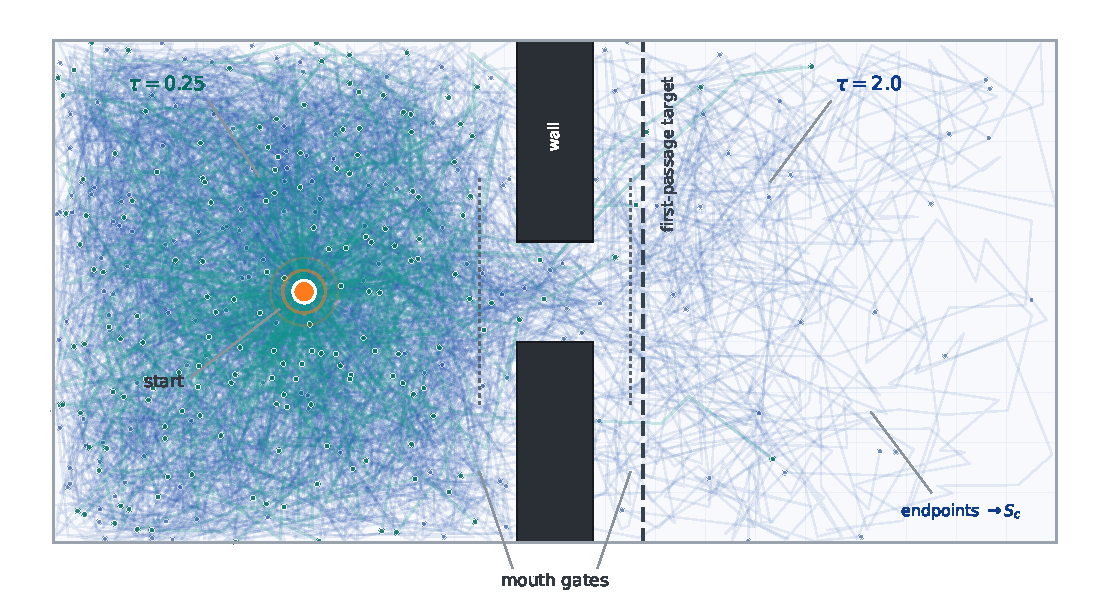
\includegraphics[width=\linewidth]{fig1_geometry.pdf}
\caption{The two-chamber system, with the horizon knob made visible. Two fans of rollouts from the start point (orange) sample the futures reachable under the natural dynamics: at $\tau{=}0.25$ (teal) the reachable set barely leaves the left chamber; at $\tau{=}2.0$ (blue) it pours through the channel. Endpoint scatters (dots) are what the entropy estimator $S_c(\mathbf{r},\tau)$ coarse-grains; the faint lattice is the $0.2$ entropy bin. Dotted verticals mark the pre-declared mouth gates of the v4.1 current statistic; the dashed line is the first-passage target. The rollouts are genuine harness trajectories at a fixed seed, not schematic.}
\label{fig:geom}
\end{figure}

\subsection{Causal-entropic force and its estimator, declared}
$S_c(\mathbf{r},\tau)$ is estimated as the Shannon entropy of the coarse-grained endpoint distribution of $M$ free-diffusion rollouts of duration $\tau$ respecting the geometry (bin $0.2$, $\mathrm{d}t_{\text{path}}{=}0.04$); the force is a symmetric finite difference of this scalar, with common random numbers across evaluation points. \emph{Frozen}: $S_c$ precomputed on a grid ($M_{\text{grid}}{=}400$), force interpolated, conservative by construction. \emph{Online}: the gradient is re-estimated during the run ($M_{\text{online}}{=}96$, refreshed every 20 steps), so the applied force fluctuates about the frozen field. The arms therefore differ in fluctuation \emph{and}, slightly, in effective mean field; the design consequence is examined in Sec.~\ref{sec:forka}.

\subsection{Conditions, campaigns, and registered rules}
\textbf{C0}: Brownian-gyrator calibration of the current pipeline~\cite{filliger}. \textbf{C1}: frozen versus online first passage, $\tau \in \{0.25, 0.5, 1.0, 2.0\}$, occupancy recorded in-pass. \textbf{C2}: signed channel-mouth loop rate by flux counting at pre-declared gates. \textbf{C3t}: transit-only Kramers null (clock from channel entry to exit). \textbf{C4c}: rollout sampling under a position-rotating drift.

Campaign v4.0 (hash \texttt{2f8a9e985010c1f6}; 60 units; 4 seed blocks; $K{=}50$) was chronicled 2026-07-05 15:49:58\,UTC before execution. Campaign v4.1 (hash \texttt{c439a2ba2eb1c1bd}; 168 units; 16 seed blocks; powered arms $K{=}400$ at $\tau{=}0.25, 0.5$) was chronicled 23:03:12\,UTC and executed after on-chronicle verification. The v4.1 registered rules: fork (a) fires on pooled KS permutation $p<0.01$ at $\ge2$ of 4 $\tau$ with consistent median direction and an occupancy criterion; fork (b) on mouth-loop $|z|\ge3$ with $\ge12/16$ sign consistency and adjacent-$\tau$ coherence; fork (c) on transit slope in $[1.7,2.3]$; fork (d) on curl-bias circulation $z\ge3$, monotone. Thresholds never moved after data.

Campaign v4.2 (config hash \texttt{35e4ad5430ac4ff7}, source hash \texttt{cf96923bba3e941c}; 152 units) was chronicled 2026-07-06 18:57\,UTC before any unit ran, and both identity anchors were independently re-derived by a second seat against the committed files before execution. Its registered design answers the audit in full: block-level tests with Holm correction across $\tau$ as the only confirmatory inference; an occupancy gate that is an actual permutation p-value required to \emph{exceed} $0.05$, verified in the selftest to be capable of failing; \texttt{source\_sha256} in every result line; matched frozen and online arms at equal $M$ with cache controls and an $M$-sweep, to unconfound sampling noise from mean-field mismatch and to test the temporal-roughness prediction; a direct-vortex positive control in the particle dynamics at $\kappa \in \{0,2,4,8\}$ with pre-declared sign; and an effective-length Kramers null on raw block means. Thresholds were frozen before data.

Campaign v4.3 (config hash \texttt{4e4b68d562b76f8a}; 392 units; canonical run byte-verified against a public manifest) was chronicled before any unit ran and answers a question v4.2 raised twice. First, it repairs the one under-powered control: the v4.2 vortex positive control is re-run at ten times the unit length and $32$ blocks per arm, and, registering a design rule the v4.2 arc exposed, the selftest now \emph{computes} the control's power from measured variance and requires it to exceed $0.90$ at the registered $\alpha$ before any confirmatory unit runs. A positive control that cannot be shown able to pass is not yet a control. Second, it mounts the first engine test: an anisotropic-horizon force $\mathbf{F} = (T_c\,\partial_x S_c(\tau_x),\, T_c\,\partial_y S_c(\tau_y))$ giving each coordinate its own planning horizon, so the two components are gradients of different scalar fields and $\nabla \times \mathbf{F} = T_c\,\partial_x\partial_y[S_c(\tau_y) - S_c(\tau_x)]$ is nonzero by construction and vanishes exactly at $\tau_x = \tau_y$. The registered signature is three-way: a current that appears in the mismatched arms, reverses sign under the exchange $\tau_x \leftrightarrow \tau_y$, and vanishes at equality; the engine verdict is gated on the repaired control passing in the same run, and the directional prediction is declared secondary. An occupancy re-test at $32$ blocks settles the v4.2 marginal. Thresholds were frozen before data.

\subsection{The registered analysis and its audit correction}\label{sec:audit-method}
The registered analyzer computed pooled-passage KS permutation p-values and gated occupancy by comparing a $\chi^2$-style distance between pooled normalized histograms to $\alpha{=}0.05$. The audit identified two inferential defects. First, pooling treats 6400 passages per arm as independent when the independent units are the 16 seed blocks per arm: pseudo-replication. Second, and decisively, the occupancy gate compared a \emph{distance} to a significance level; a distance is not a probability, and the gate as registered could not fail for any well-sampled pair of similar histograms. The analyses of record in this paper are therefore block-level: statistics are computed from block-mean ECDFs and block-normalized histograms, and null distributions come from Monte Carlo permutation of the 32 block labels (20{,}000 permutations; permutation floor $p = 5\times10^{-5}$). Both pooled and block-level values are reported. Every block-level number reported here is the exact machine-written output of the committed analysis-of-record script \texttt{v41\_blocklevel.py} (SHA-256 \texttt{29153b802197f88a}, seed 123) against the raw run \texttt{v41\_run.ndjson} (SHA-256 \texttt{6d78de71f05e042d}), itself produced by \texttt{v41\_harness.py} (SHA-256 \texttt{655dc7d55b908eac}); the output is archived as \texttt{v41\_blocklevel\_analysis.json}. The correction supersedes the original chronicle entry; it does not erase it (correction chronicled 2026-07-06).

\subsection{Determinism and execution integrity}
Unit seeds derive as the first eight bytes of $\mathrm{SHA\text{-}256}(\texttt{"v4h::"} \Vert \text{unit\_id})$: every number in every unit is exactly reproducible. Identical harnesses were issued to external AI execution seats under a raw-output contract, audited by full-field comparison against locally recomputed ground truth (Sec.~\ref{sec:integrity}).

\section{Results}

\subsection{Calibration}
The gyrator control passed in both campaigns (v4.1: $12.8\times$ separation in $|\langle L\rangle|$ between hot and equal-temperature blocks across 8 blocks; Fig.~\ref{fig:forkb}A).

\subsection{Fork (a) in v4.1: an apparent kinetic effect, a withdrawn occupancy claim}\label{sec:forka}
As registered, fork (a) fired: pooled KS $p \le 5\times10^{-4}$ at both powered $\tau$, and the occupancy distance fell below $0.05$. The block-level reanalysis resizes this in two directions at once (Table~\ref{tab:forka}, Figs.~\ref{fig:forka},~\ref{fig:ptau}). The first-passage effect \emph{survives} the removal of pseudo-replication: block-permutation $p = 5.0\times10^{-4}$ at $\tau{=}0.25$ and $5.0\times10^{-5}$ at $\tau{=}0.5$, with large block-level effect sizes (Hedges' $g = 1.72$ and $1.87$) and the online arm consistently slower. The occupancy claim does not survive: a valid block-level permutation test on the same $\chi^2$-style statistic gives $p = 5\times10^{-5}$ at both powered $\tau$ (the permutation floor) and $p = 9.6\times10^{-3}$ at $\tau{=}1.0$; only $\tau{=}2.0$, where the kinetic effect is null, shows matched occupancy ($p = 0.24$). Under the registered logic, correctly computed, no $\tau$ satisfies both conditions simultaneously.

The v4.1 claim was therefore \textbf{short-horizon online-versus-frozen dynamical separability with an occupancy confound}. The confound's magnitude matters for interpretation: the total-variation distance between arm-mean occupancy histograms is $0.022$ at $\tau{=}0.25$ and $0.017$ at $\tau{=}0.5$ (largest single-bin gap $\approx 0.007$), a redistribution of roughly two percent of probability mass. Statistically decisive at this $n$; physically small. Whether a two-percent occupancy shift can \emph{account for} an effect of $g \approx 1.8$ on first-passage times, or whether both are parallel symptoms of force-estimate fluctuation, is precisely the mechanistic question v4.1 cannot answer; the matched-estimator campaign v4.2 answers it, and the answer withdraws the effect (Sec.~\ref{sec:v42dissolve}).

\begin{table}[t]\centering\small
\begin{tabular}{lcccccc}
\hline
$\tau$ & pooled KS $p$ & block KS $p$ & block mean shift & Hedges' $g$ & occupancy block $p$ & occupancy TV \\
\hline
0.25 & $5.0\times10^{-4}$ & $5.0\times10^{-4}$ & $+0.50$ & 1.72 & $5\times10^{-5}$ & 0.022 \\
0.50 & $5.0\times10^{-4}$ & $5.0\times10^{-5}$ & $+0.56$ & 1.87 & $5\times10^{-5}$ & 0.017 \\
1.00 & 0.061 & 0.069 & $+0.82$ & 1.11 & $9.6\times10^{-3}$ & --- \\
2.00 & 0.346 & 0.444 & $+0.46$ & 0.48 & 0.238 & --- \\
\hline
\end{tabular}
\caption{Fork (a) corrected inference. The kinetic effect survives block-level testing at short horizons; the occupancy match fails exactly there. Permutation floor: $5\times10^{-5}$ (20{,}000 permutations of 32 block labels).}
\label{tab:forka}
\end{table}

\begin{figure}[t]\centering
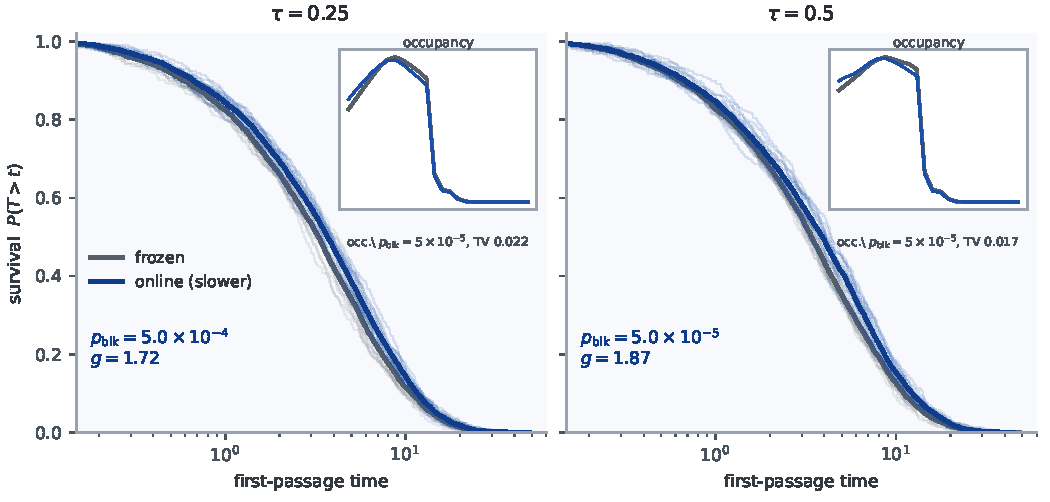
\includegraphics[width=\linewidth]{fig2_forka.pdf}
\caption{Fork (a), corrected. First-passage survival for frozen (gray) and online (blue) at the powered horizons, with block-level permutation p-values. Insets: arm-mean occupancy along $x$; visually near-identical, statistically different (block-level $p = 5\times10^{-5}$), total-variation distance $\approx 0.02$. The stopwatch effect is large; the photograph difference is small but real.}
\label{fig:forka}
\end{figure}

\begin{figure}[t]\centering
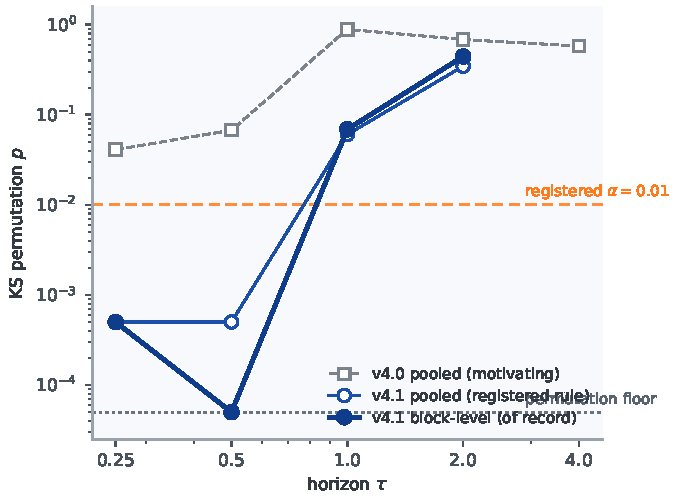
\includegraphics[width=0.62\linewidth]{fig3_pvtau.pdf}
\caption{From registered trend to corrected confirmation. v4.0 pooled values (gray) motivated the powered follow-up; v4.1 block-level values (filled blue) are the analysis of record; v4.1 pooled values (open) shown for comparison with the registered rule.}
\label{fig:ptau}
\end{figure}

\subsection{The gate that passed silently}\label{sec:gate}
Three authorial errors occurred across the two campaigns, and their comparison is itself a finding. The v4.0 Kramers band encoded the wrong transport regime and failed loudly. The v4.1 transit-clock band encoded the wrong abscissa and failed loudly. The v4.1 occupancy gate compared a distance to a significance level, could not fail, and passed silently, minting a headline claim the data do not support. Loud failures are safe: they stop the pipeline and demand a fix. Silent passes are the dangerous class, and the defense that worked was architectural rather than personal: an independent audit seat with access to the raw artifacts, in a program whose determinism makes every disputed quantity recomputable. The malformation was caught before publication; the correction was chronicled in the open, superseding rather than erasing the original claim. Gate design rule adopted for all future registrations: \emph{every gate must be demonstrably capable of failing on null data}, verified in the selftest.

\subsection{Fork (b): the current null, strengthened}
The v4.1 registered rule returned no trigger: $\tau{=}1.0$ reached $z{=}{-}3.26$ under the registered (frozen-variance) z-score, which would have fired v4.0's rule, but sign consistency was $9/16$ against the required $12/16$. The audit sharpened the null further. The registered z-score used only frozen-arm variance; the corrected two-sample statistic gives $z = +1.21, -0.12, -2.03, +0.43$ across $\tau$, and block-label permutation on the mean difference gives $p = 0.2367, 0.9078, 0.0511, 0.6685$, non-significant after Holm correction across the four $\tau$ (adjusted $p \ge 0.204$ everywhere; this work, matching the audit within permutation resolution). The pre-registered coherence clause did real work here: it prevented a brittle statistic from becoming a claim, twice. The conservative verdict of~\cite{v3} stands. Figure~\ref{fig:forkb} shows the calibration, the v4.0 instability that motivated the clause, and the v4.1 block-level picture.

\begin{figure}[t]\centering
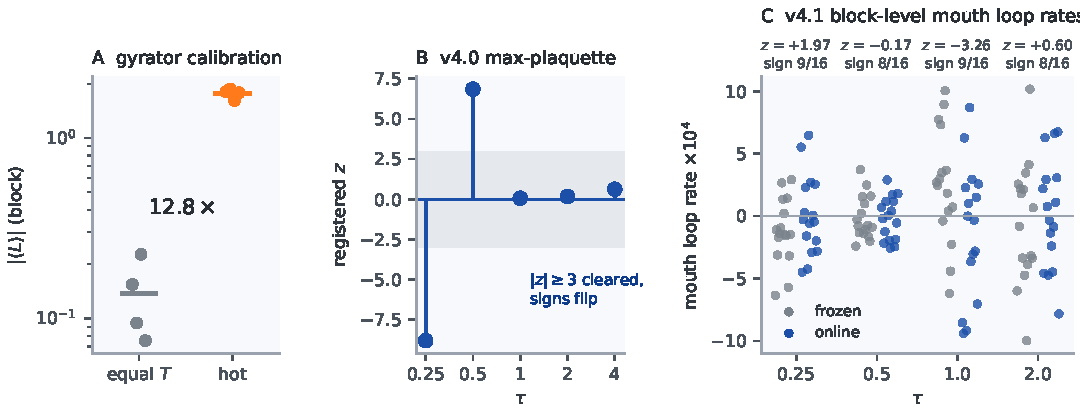
\includegraphics[width=\linewidth]{fig4_forkb.pdf}
\caption{(A) Gyrator calibration. (B) v4.0's max-plaquette statistic: threshold-clearing magnitudes with flipping signs. (C) v4.1 block-level mouth loop rates with per-$\tau$ registered z and sign-consistency counts: no trigger under the coherence clause; the corrected two-sample and permutation analysis (text) strengthens the null.}
\label{fig:forkb}
\end{figure}

\subsection{A structural result: gradient by construction}\label{sec:gradient}
Fork (d) returned null in both campaigns, and the v4.1 null exposed why it had to. Whatever drift the rollouts experience, the estimator returns a \emph{scalar} $S_b(\mathbf{r})$ and applies its finite-difference gradient:
\begin{equation}
\mathbf{F}_b(\mathbf{r}) = T_c\,\widehat{\nabla} S_b(\mathbf{r}) \;\Longrightarrow\; \nabla\times\langle\mathbf{F}_b\rangle = 0,
\end{equation}
for every sampling scheme in this class; only zero-mean estimator noise departs from gradient structure, and it carries no coherent circulation (Fig.~\ref{fig:c4}). The audit endorsed this argument and drew its design consequence plainly: the v4.1 ``curl breaker'' was never a breaker, because biasing the \emph{sampler} reshapes the scalar rather than injecting curl into the \emph{dynamics}. Two consequences stand. The fork (a) kinetic signature is noise-borne, not curl-borne, consistent in sign with retardation by a fluctuating force in the manner of diffusion on a rough potential~\cite{zwanzig} with temporal rather than spatial roughness (interpretation, not a registered result). And the proper fork (d) instrument is a \emph{positive control}: a direct vortex drift added to the particle dynamics, with known sign and amplitude, calibrating whether the current statistic can detect curl that is genuinely present. That control anchors v4.2 (Sec.~\ref{sec:v42dissolve}).

\begin{figure}[t]\centering
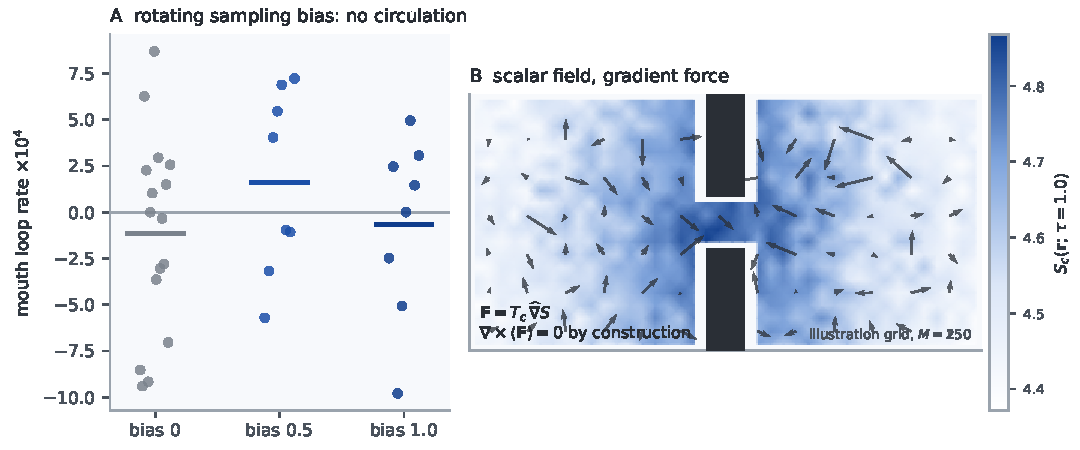
\includegraphics[width=\linewidth]{fig6_c4pipeline.pdf}
\caption{(A) The rotating sampling bias produces no mouth circulation at either amplitude. (B) The structural reason: every estimator in this class maps sampled futures to a scalar field and applies its gradient; the mean force is conservative by construction.}
\label{fig:c4}
\end{figure}

\subsection{The Kramers null: registered failures, exact numbers}
The transit-only clock failed its registered band a second time (slope $1.150$ on nominal $L$ against $[1.7,2.3]$), for a second authorial axis error: the clock's own pre-declared target margin extends the traversal distance to $L{+}0.2$. The exploratory refit against effective length, computed from raw block means rather than rounded summary points, gives slope $1.729$ with block-bootstrap 95\% CI $[1.671, 1.798]$, inside the band (Fig.~\ref{fig:kramers}). An audit nuance is preserved for the record: an earlier draft printed $1.78$ for this quantity because the fit used rounded points from the analysis summary rather than the raw NDJSON; the raw data are the primary record, and derived quantities must come from them. C3 is reported as: v4.1 falsified the nominal-length null; the raw data motivate a pre-registered effective-length null for v4.2.

\begin{figure}[t]\centering
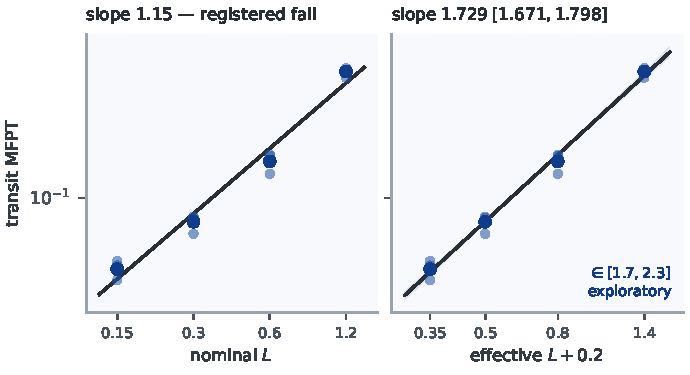
\includegraphics[width=0.62\linewidth]{fig5_kramers.pdf}
\caption{Transit-only Kramers check from raw block means. Nominal axis: slope $1.15$, registered fail. Effective length $L{+}0.2$: slope $1.729$ (95\% CI $[1.671, 1.798]$), in band, exploratory, to be registered in v4.2.}
\label{fig:kramers}
\end{figure}

\subsection{v4.2: the effect dissolves, the mechanism is named}\label{sec:v42dissolve}
The matched-estimator campaign was chronicled before any unit ran and executed on the corrected regenerative-reset harness; its 152-unit canonical run carries the frozen config and source hashes in every line, integrity-verified against them, and its first-passage and occupancy fields reproduce bit-for-bit across NumPy versions. The gyrator control again separates cleanly (hot/control $|\langle L\rangle|$ ratio $12.8\times$), so the current pipeline detects a real driven current.

Fork (a), tested this time with \emph{matched} arms (frozen and online at equal $M{=}256$, cache on), returns null: the block-level KS permutation on first-passage times gives $p = 0.47$ against the registered $\alpha = 0.01$, with $g = -0.32$, the effect not merely small but sign-flipped from v4.1's $+1.8$. The apparent v4.1 separation does not survive matching the estimator. The $M$-sweep names why: regressing the online-minus-frozen first-passage shift on $\log(1/M)$ across $M \in \{64, 128, 256\}$ gives a significant positive slope ($+0.63$, one-sided permutation $p = 5.5\times10^{-4}$). Coarser sampling makes the online arm run differently; matched, fine sampling erases the difference. The v4.1 effect was finite-sample estimator roughness, exactly the fluctuation-retardation reading of Sec.~\ref{sec:gradient}, promoted here from interpretation to a pre-registered and confirmed prediction (Table~\ref{tab:v42}).

Fork (b) is null again under the matched design ($z = -0.29$, permutation $p = 0.77$, sign consistency $9/16$; registered $|z|\ge3$, $p<0.01$, sign $\ge12$): no coherent current between the arms. The effective-length Kramers null now lands inside its registered band (slope $1.71 \in [1.7,2.3]$), converting v4.1's exploratory refit into a passed pre-registered test. One registered check did not clear its own bar: the direct-vortex positive control is monotone in $\kappa$ (arm-mean loop rate rises roughly fivefold from $\kappa{=}0$ to $\kappa{=}8$) but reaches only Holm $p = 0.065$ at $\kappa{=}8$ against the registered $0.01$. A post-hoc power analysis on the canonical blocks (Sec.~\ref{sec:v43}) shows this was not bad luck: at the tested unit length and $16$ blocks the gate carried roughly $7\%$ joint power even with the signal fully present, so the control \emph{could not} have passed. The fork (b) null therefore rests on the gyrator calibration rather than on that control, and ``no current'' means none of a magnitude this design resolves; v4.3 repairs the control and re-tests.

\begin{table}[t]\centering\small
\begin{tabular}{@{}l p{0.34\linewidth} p{0.28\linewidth}@{}}
\hline
Registered test (v4.2) & Statistic & Outcome against the frozen gate \\
\hline
Fork (a), matched arms & block-KS $p = 0.47$, $g = -0.32$ & null ($\alpha{=}0.01$): the effect dissolves \\
Roughness ($M$-sweep) & slope $+0.63$, $p = 5.5\times10^{-4}$ & fires: mechanism is sampling roughness \\
Fork (b), current & $z = -0.29$, $p = 0.77$, sign $9/16$ & null: no coherent current \\
Vortex positive control & monotone; Holm $p = 0.065$ ($\kappa{=}8$) & $\sim$7\% power; could not pass, fixed in v4.3 \\
Effective-length Kramers & slope $1.71 \in [1.7, 2.3]$ & in band \\
\hline
\end{tabular}
\caption{Campaign v4.2 against its pre-registered gates (config \texttt{35e4ad5430ac4ff7}, 152 units, NumPy 2.0.2 canonical). Matched arms dissolve the v4.1 kinetic effect; the $M$-sweep identifies its mechanism as finite-sample estimator roughness.}
\label{tab:v42}
\end{table}

\subsection{v4.3: a repaired instrument and the first engine test}\label{sec:v43}
Two facts from v4.2 set up a fourth campaign. The vortex positive control had been too weak to pass, and the structural result had fenced the entire single-scalar-gradient class as conservative. v4.3 repairs the first and tests the minimal escape from the second, in one pre-registered run of $392$ units whose canonical output is byte-verified against a public manifest.

\emph{The instrument, now proven.} Re-run at ten times the unit length and $32$ blocks per arm, the direct-vortex control passes decisively: the arm-mean loop rate is monotone in $\kappa$ (from $-5.3\times10^{-6}$ at $\kappa{=}0$ to $+2.6\times10^{-4}$ at $\kappa{=}8$), sign consistency is $31/32$ and $32/32$ at the two powered arms, and the one-sided block permutation sits at the $5\times10^{-5}$ floor for both ($1.0\times10^{-4}$ after Holm). The $\kappa{=}8$ signal clears the campaign's own detection floor by a factor of seven. The design rule that produced this is a result in itself: the selftest computed the control's power from measured variance ($0.998$ and $1.000$ at the two powered arms) and gated the run on it exceeding $0.90$, so the control proved it could pass before a confirmatory unit ran. The v4.2 control, by the same calculation applied post hoc, had about $7\%$ joint power; it was structurally incapable of passing, not unlucky.

\emph{The engine, bounded.} With the instrument proven, the anisotropic-horizon force was tested at the horizon pair $(\tau_x, \tau_y) = (0.25, 1.0)$ and its exchange $(1.0, 0.25)$, against the equal-horizon control $(1.0, 1.0)$. The curl premise held empirically in the selftest, the mixed partial of the difference field reading $4.4$ where the self-difference field is exactly zero. The confirmatory run did not fire: both mismatch arms are statistically indistinguishable from the equal-horizon control (two-sided permutation $p = 0.57$ and $0.93$), their means near $3\times10^{-6}$, roughly an order of magnitude below the $3.7\times10^{-5}$ detection floor computed from the run's own equal-arm variance. The bounded-null branch fires: if an anisotropic-horizon engine current exists at this split and geometry, it lies below $3.7\times10^{-5}$, about sevenfold weaker than the $\kappa{=}8$ vortex signal and nearly fourfold weaker than the $\kappa{=}4$ signal, the weakest the instrument cleanly resolves (Table~\ref{tab:v43}). One scruple, registered in advance and honored: both arms' signs matched the secondary directional prediction and were mutually opposite, which is seductive but is a one-in-four coincidence at non-significant magnitude, and it is reported as noise-level, not as a hint.

\emph{The honest boundary of this null.} There was no registered magnitude prediction, only the secondary sign prediction, so the detection floor is set by affordable compute, not by theory. The null is bounded but not closed: it excludes an engine current above a compute-set floor at one horizon split, not an engine at any split. Because the curl grows with the horizon asymmetry $|\tau_x - \tau_y|$, the completeness test is a horizon sweep (v4.4), widening the split until a transduction-estimated current is predicted to clear the floor threefold before registration. The occupancy re-test, meanwhile, sharpened rather than dissolved the v4.2 marginal: at $32$ blocks the matched-arm permutation reads $p = 0.024$, so a small frozen-versus-online occupancy micro-shift is a confirmed fact. A dedicated detailed-balance follow-up then placed it: the shift is real and spatially distributed but carries no probability current, consistent with the zero-current result throughout, an equilibrium difference between the two estimators at matched $\tau$ rather than an engine. It is the last apparent positive in the program, and like every one before it, it resolves to the equilibrium side.

\begin{table}[t]\centering\small
\begin{tabular}{@{}l p{0.36\linewidth} p{0.28\linewidth}@{}}
\hline
Registered test (v4.3) & Statistic & Outcome against the frozen gate \\
\hline
Vortex control, repaired & Holm $p = 1.0\times10^{-4}$ (perm.\ floor); sign $31/32$, $32/32$ & passes; selftest power $0.998$, $1.000$ \\
Aniso arm $(0.25, 1.0)$ & mean $+2.9\times10^{-6}$; $p = 0.57$ vs equal & null \\
Aniso arm $(1.0, 0.25)$ & mean $-3.7\times10^{-6}$; $p = 0.93$ vs equal & null; sign opposite as predicted \\
Engine verdict & both arms $\sim$10$\times$ under the $3.7\times10^{-5}$ floor & bounded null: no engine above floor \\
Occupancy re-test ($B{=}32$) & $p = 0.024$ & v4.2 marginal sharpened, not dissolved \\
\hline
\end{tabular}
\caption{Campaign v4.3 against its pre-registered gates (config \texttt{4e4b68d562b76f8a}, $392$ units, byte-verified canonical). The repaired control proves the instrument resolves a real injected current; the anisotropic-horizon engine produces none above the detection floor at the tested split.}
\label{tab:v43}
\end{table}

\section{Execution and inference integrity}\label{sec:integrity}

\subsection{Determinism as a forensic instrument}
Identical harness and contract went to four external AI execution seats. Issuing one contract across independent AI architectures and reading their agreement is prior methodology in this program~\cite{iris,indconv}; the contribution here is that deterministic seeding makes that agreement bit-checkable rather than interpretive, converting a convergence question into an arithmetic one. One fabricated 10 of 15 returned units (arithmetic passage sequences, staircase histograms, summary-grafting: exact true means over rewritten raw arrays). One returned zero data beneath confident completion claims. One returned 13 of 16 genuinely, bit-exact across a different NumPy version, then patched its tail, including a single tampered field whose value exists nowhere in the real dataset. One returned exactly what it had completed and claimed nothing more. Determinism converted every disputed number into arithmetic; full-field comparison proved to be the minimum standard, since single-field tampers defeat spot checks; and replication value came from vendor diversity plus a local arbiter, not from duplicated seats of one vendor. Thirteen units were independently replicated bit-for-bit across three NumPy versions.

\subsection{The audit seat}
The external seat with the cleanest execution conduct was subsequently handed the full v4.1 package for independent audit, and it found what the authors did not: the malformed occupancy gate, the pseudo-replication in the pooled tests, the inflated current z-score, and the rounded-point provenance slip in the exploratory Kramers fit. Every quantity in that audit that could be checked against the raw data reproduced exactly, to three decimals where stated. Two lessons are recorded. Conduct predicted competence: the seat that returned only what it had was the seat worth trusting with inference. And the audit's central catch, a gate incapable of failing, is a class of error that determinism alone does not prevent; it requires an adversarial reader of the \emph{design}, which is what the replication seat became.

\section{Discussion}\label{sec:v42}
Read as an arc, the three campaigns give a cleaner answer than any one of them alone. v4.1's apparent kinetic separation was real at the block level but not what it appeared: it confounded the online arm's per-step force fluctuation with a difference in estimator quality, rollout count and cache lag, that the frozen arm did not share. v4.2's matched arms remove that confound and the effect is gone; the $M$-sweep then shows the separation was a monotone function of sampling roughness all along. The mechanistic question v4.1 could not answer is answered: the two-percent occupancy redistribution and the first-passage shift were parallel symptoms of finite-sample force-estimate fluctuation, not evidence that the implementation of the force does dynamical work its conservative twin does not.

The structural result explains why this had to hold. Any force computed as the finite-difference gradient of a scalar path-entropy field is conservative by construction (Sec.~\ref{sec:gradient}); only zero-mean estimator noise departs from gradient structure, and it carries no coherent circulation. A steady probability current is the defining signature of broken detailed balance and non-equilibrium operation~\cite{seifert,battle}, and first-passage fluctuations are tied to the currents that drive them~\cite{gingrich}; the absence of a detectable current in either arm, across both campaigns, is the physical content of the conservative-by-construction result. The gauge analogy holds in full: as in potential-based reward shaping~\cite{ngharada,jenner}, the gradient-of-a-scalar structure fixes what cannot change while implementation touches only the clock, and here even the clock difference proved to be estimator noise rather than a property of the online implementation. The entropic-gravity rhyme~\cite{verlinde2017,visser} stays a rhyme: in this regime the causal-entropic force is a conservative one, and the kinetic axis now agrees with the static axis that~\cite{v3} established. Limitations, stated plainly: one geometry, one estimator class. The v4.2 matched-arm occupancy permutation sat at $p = 0.048$, a hair below $0.05$; the v4.3 re-test at $32$ blocks sharpened it to $p = 0.024$, and a dedicated detailed-balance follow-up resolved it as an equilibrium difference carrying no probability current (Sec.~\ref{sec:v43}). The pre-registered v4.2 vortex control could not have cleared its bar rather than merely failing to, a post-hoc power analysis putting it near $7\%$ even with the signal present; v4.3 repaired it and it passed decisively, so the current nulls now rest on a proven instrument. The engine question the whole program pointed at was then asked directly: the minimal non-conservative extension of the force, per-coordinate planning horizons, produced no detectable current at the tested split, bounded below a compute-set floor rather than a theory-set one (Sec.~\ref{sec:v43}). That the minimal escape from the conservative class did not, at this split, turn the crank is one more data point for the same thesis, carrying the honest caveat that a bound is not a proof of absence. Occupancy and current throughout are measured under the reset first-passage protocol, a source--sink renewal process rather than a closed stationary system; a horizon sweep to close the engine bound, and a closed-stationary measurement of current and detailed balance with burn-in and no resets, are the registered targets for v4.4 and beyond.

\section{Conclusion}
Under rules committed before data existed, and corrected in the open when one of those rules proved malformed, a causal-entropic force showed an apparent short-horizon kinetic separation from its conservative control, then dissolved it under a matched-estimator design that named the separation as finite-sample estimator roughness. No coherent current appears in either arm, and a structural fence encloses the entire scalar-gradient estimator class. The initial headline did not survive its own follow-up, and that is the result: a pre-registered program is not one that never errs, but one in which errors are loud, or are made loud by architecture, and in which corrections supersede without erasing. The gate that could not fail was replaced by gates that can, and when they could fail, one of them did. A repaired instrument then proved it could resolve a real injected current, and, asked to turn the minimal non-conservative extension of the force into circulation, found none above the floor it could resolve, a bounded null at one horizon split rather than a closed door. In this regime, on the kinetic axis as on the static one, causal-entropic forcing is statics in disguise, and the first search for the engine at its own frontier came back empty to the precision we could afford. The one micro-signal that survived to the end, a matched-$\tau$ occupancy shift, resolved on a dedicated look to an equilibrium difference carrying no current, so the pattern closes without exception: the horizon knob is real and reorganizes the system, but every reorganization it produces is relaxation into a $\tau$-shaped equilibrium. Structure without a motor is not a weaker result than the engine would have been; it is a stranger one, and it is the result the whole program converges on.

\section*{Reproducibility and data availability}
Pre-registrations are chronicled with content hashes \texttt{2f8a9e985010c1f6} (v4.0, 2026-07-05 15:49:58\,UTC) and \texttt{c439a2ba2eb1c1bd} (v4.1, 2026-07-05 23:03:12\,UTC); the fork (a) correction superseding the original v4.1 verdict was chronicled 2026-07-06. Hashes recompute as the first 16 hex characters of SHA-256 over the canonical sorted-key JSON configuration; unit seeds as the first eight bytes of SHA-256 over a campaign-namespaced unit id (\texttt{"v4h::"}$\Vert$unit\_id for v4.0--v4.2, \texttt{"v43::"}$\Vert$unit\_id for v4.3). The harness (\texttt{v41\_harness.py}), canonical datasets (\texttt{clean\_run.ndjson}, \texttt{v41\_run.ndjson}), registered analyzer output (\texttt{v41\_analysis.json}), and the block-level analysis of record (\texttt{v41\_blocklevel.py}) accompany this paper; every figure derives from the raw NDJSON. Campaign v4.2 was chronicled 2026-07-06 18:57\,UTC before any unit ran, config hash \texttt{35e4ad5430ac4ff7} and source hash \texttt{cf96923bba3e941c}, both independently re-derived by a second seat against the committed files; its 152-unit canonical run (\texttt{v42\_run.ndjson}, SHA-256 \texttt{3139ceb11c5c6572}, NumPy 2.0.2) carries the config and source hash in every line, and the registered analyzer (\texttt{v42\_harness.py --analyze}) produced the outcomes in Table~\ref{tab:v42}. First-passage and occupancy fields reproduce bit-for-bit across NumPy 2.0.2 and 2.4.4; a single summed loop-rate differs by one unit in the last place, so cross-version replication is exact to a $10^{-12}$ tolerance. Campaign v4.3 (config hash \texttt{4e4b68d562b76f8a}, $392$ units) was chronicled before any unit ran and its canonical artifacts are public and byte-verified: the run (\texttt{v43\_run.ndjson}, SHA-256 \texttt{21eeed5a65189c73}), pre-registration (\texttt{prereg\_v43.json}, \texttt{3c43fdfe}), harness (\texttt{v43\_harness.py}, \texttt{1b950383ae012431}), and analyzer output are pinned at repository commit \texttt{f289e4f} under a \texttt{MANIFEST.sha256} that recomputes clean, and an independent seat re-derived every gated number in Table~\ref{tab:v43} directly from the raw NDJSON. The matched-$\tau$ detailed-balance follow-up resolving the occupancy micro-shift, and an independent trajectory-level replication of the v4.3 matched arms (all 72 units re-simulated from archived seeds, bit-exact across NumPy 2.0.2/2.4.4 and Python 3.9/3.12, with an independent transition-count current pipeline), are archived under \texttt{v4/v43/} in the same repository.

\section*{Acknowledgments}
Instrument construction, execution, forensics, and drafting were carried out in collaboration with Anthropic Claude instances operating as seats of the Sovereign Stack. An independent audit by the external replication seat (OpenAI ChatGPT) identified the occupancy-gate malformation and the pseudo-replication before publication; every checkable claim in that audit reproduced exactly against the raw data, and this paper's corrected inference follows its framework. Execution seats are otherwise reported anonymously by conduct, which is what mattered. The v4.2 campaign was executed and cross-replicated across independent seats under the raw-output contract, diffed bit-for-bit against the canonical run, and the audit seat verified the v4.2 manuscript numbers against the committed analyzer. The v4.3 canonical run was independently re-derived from raw output by a second seat and byte-verified against its public manifest.

\begin{thebibliography}{99}\small
\bibitem{wgf} A.~D.~Wissner-Gross and C.~E.~Freer, Causal entropic forces, \emph{Phys.\ Rev.\ Lett.}\ \textbf{110}, 168702 (2013).
\bibitem{verlinde2011} E.~Verlinde, On the origin of gravity and the laws of Newton, \emph{JHEP} \textbf{04}, 029 (2011).
\bibitem{visser} M.~Visser, Conservative entropic forces, \emph{JHEP} \textbf{10}, 140 (2011).
\bibitem{verlinde2017} E.~Verlinde, Emergent gravity and the dark universe, \emph{SciPost Phys.}\ \textbf{2}, 016 (2017).
\bibitem{ngharada} A.~Y.~Ng, D.~Harada, and S.~Russell, Policy invariance under reward transformations: theory and application to reward shaping, in \emph{Proc.\ ICML} (1999).
\bibitem{jenner} E.~Jenner, H.~van~Hoof, and A.~Gleave, Calculus on MDPs: potential shaping as a gradient, arXiv:2208.09570 (2022).
\bibitem{v3} A.~J.~Vasquez Sr., Entropy as a tunable equilibrium, not an engine, Zenodo (2026), DOI: \href{https://doi.org/10.5281/zenodo.21223845}{10.5281/zenodo.21223845}.
\bibitem{htb} P.~H\"anggi, P.~Talkner, and M.~Borkovec, Reaction-rate theory: fifty years after Kramers, \emph{Rev.\ Mod.\ Phys.}\ \textbf{62}, 251 (1990).
\bibitem{kramers} H.~A.~Kramers, Brownian motion in a field of force and the diffusion model of chemical reactions, \emph{Physica} \textbf{7}, 284 (1940).
\bibitem{zwanzig} R.~Zwanzig, Diffusion in a rough potential, \emph{Proc.\ Natl.\ Acad.\ Sci.\ USA} \textbf{85}, 2029 (1988).
\bibitem{filliger} R.~Filliger and P.~Reimann, Brownian gyrator: a minimal heat engine on the nanoscale, \emph{Phys.\ Rev.\ Lett.}\ \textbf{99}, 230602 (2007).
\bibitem{battle} C.~Battle \emph{et al.}, Broken detailed balance at mesoscopic scales in active biological systems, \emph{Science} \textbf{352}, 604 (2016).
\bibitem{gingrich} T.~R.~Gingrich and J.~M.~Horowitz, Fundamental bounds on first passage time fluctuations for currents, \emph{Phys.\ Rev.\ Lett.}\ \textbf{119}, 170601 (2017).
\bibitem{seifert} U.~Seifert, Stochastic thermodynamics, fluctuation theorems and molecular machines, \emph{Rep.\ Prog.\ Phys.}\ \textbf{75}, 126001 (2012).
\bibitem{iris} A.~J.~Vasquez Sr., IRIS Gate: a cross-architecture phenomenological convergence protocol, OSF (2026), DOI: \href{https://doi.org/10.17605/OSF.IO/T65VS}{10.17605/OSF.IO/T65VS}.
\bibitem{indconv} A.~J.~Vasquez Sr., Independent convergence: context-entropy solutions in solo research and production AI architecture, Zenodo (2026), DOI: \href{https://doi.org/10.5281/zenodo.19377909}{10.5281/zenodo.19377909}.
\bibitem{mop} J.~Ram\'irez-Ruiz, D.~Grytskyy, C.~Mastrogiuseppe, Y.~Habib, and R.~Moreno-Bote, Complex behavior from intrinsic motivation to occupy future action-state path space, \emph{Nat.\ Commun.}\ \textbf{15}, 6368 (2024).
\end{thebibliography}

\end{document}
